\subsection{Transformacija podatkov}

\begin{minipage}{0.45\textwidth}
    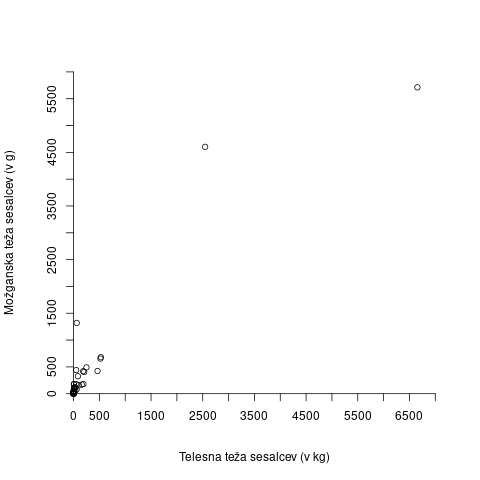
\includegraphics[width=1\textwidth]{res/netrans-razsevni-diagram.png}
    \captionof{figure}{Razsevni diagram\\(netransformiran)}
    \label{img:netrans-razsevni-diagram}
\end{minipage}
\hfill
\begin{minipage}{0.55\textwidth}
    Ob analizi razsevnega diagrama telesne teže sesalcev v primerjavi z velikostjo njihovih možganov
    (glej graf \ref{img:netrans-razsevni-diagram}) lahko opazimo, da podatki ne sledijo linearni zvezi.
    R ukaz \verb|(cor(mozgani$telteza, mozgani$moteza))|, ki izračuna korelacijski koeficient podanih spremenljivk,
    nam vrne rezultat \verb|[1] 0.9340911|, kar pomeni, da so podatki korelirani, tako da lahko vseeno nadaljujemo
    njihovo analizo, a jih moramo prvo transformirati.
    Podatke lahko transformiramo z logaritemsko funkcijo, pri čemer na razsevnem diagramu (glej graf \ref{img:razs-diag})
    opazimo, da so v tem primeru logaritmi podatkov linearno zvezni.
\end{minipage}
\\

Na grafu linearnosti modela (glej graf \ref{img:netrans-linearnost-modela}) je razvidno, da so točke zgoščene na levi
strani grafa, kar nakazuje na nelinearnost originalnega modela (pred transformacijo).

Na grafu normalnosti porazdelitve (glej graf \ref{img:netrans-normalnost-porazdelitve}) lahko opazimo odstopanja od
regresijske premice, a ne tako velika, da bi kazala na problem ujemanja podatkov z netransformiranim modelom.

Na grafu homogenosti variance (glej graf \ref{img:netrans-diagnosticni-grafi}) lahko opazimo, da so točke
zgoščene na levi strani, prav tako pa vidimo, da varianca naraste, zato zanjo ne moremo reči, da je homogena.

Na grafu vpliva točk na model (glej graf \ref{img:netrans-vpliv-tock-na-model}) lahko takoj opazimo tri točke z
največjo Cookovo razdaljo, 16., 29. in 30. podatkovno točko.

Da preverimo, če podatkovne točke zelo vplivajo na model, uporabimo spodnje ukaze:

\begin{verbatim}
    which(cooks.distance(model) > 4/57)
    any(cooks.distance(model)[c(16)] >= qf(0.5, 2, 57))
    any(cooks.distance(model)[c(29)] >= qf(0.5, 2, 57))
    any(cooks.distance(model)[c(30)] >= qf(0.5, 2, 57))
\end{verbatim}

pri čemer nam prvi ukaz vrne rezultat \emph{16, 29, 30}, zato smo zagnali tudi spodnje tri ukaze, kjer nam odgovora
za točki 16 in 30 vrneta rezultat \verb|[1] TRUE|, odgovor za točko 19 pa rezultat \verb|[1] FALSE|.
Ti rezultati nam povejo, da 16. in 30. podatkovna točka močno vplivata na linearnost modela, zato bi ju morali pred
nadaljevanjem odstraniti, a ker model na podlagi prejšnjih opažanj iz diagnostičnih grafov ne zadošča predpostavkam
linearnega modela, moramo podatke pred nadaljevanjem transformirati.

\newpage

\begin{figure}[h]
    \centering
    \begin{subfigure}[ht]{0.49\textwidth}
        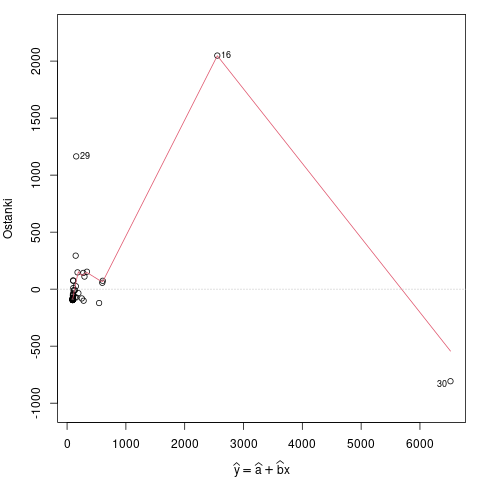
\includegraphics[width=1\textwidth]{res/netrans-linearnost-modela.png}
        \captionof{figure}{Linearnosti modela\\(netransformiran)}
        \label{img:netrans-linearnost-modela}
    \end{subfigure}
    \hfill
    \begin{subfigure}[ht]{0.49\textwidth}
        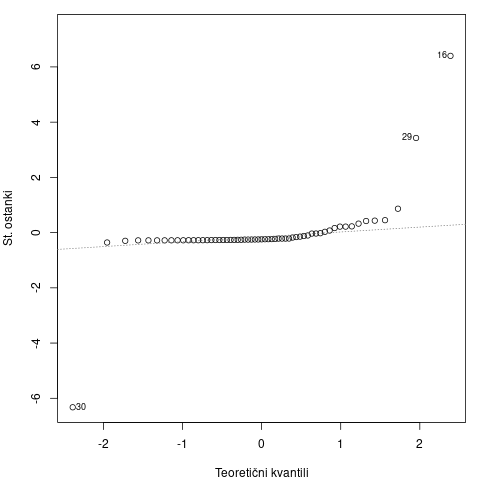
\includegraphics[width=1\textwidth]{res/netrans-normalnost-porazdelitve.png}
        \captionof{figure}{Normalnost porazdelitve\\(netransformiran)}
        \label{img:netrans-normalnost-porazdelitve}
    \end{subfigure}

    \begin{subfigure}[ht]{0.49\textwidth}
        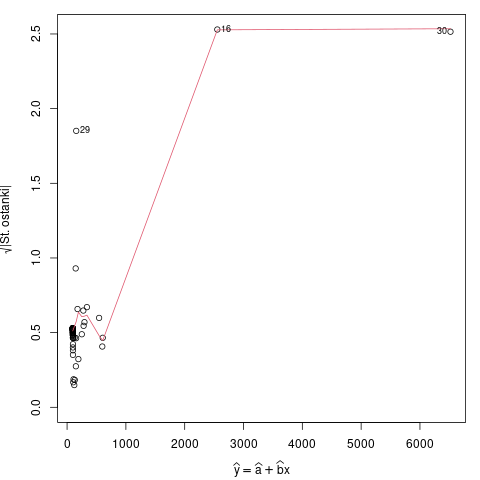
\includegraphics[width=1\textwidth]{res/netrans-homogenost-variance.png}
        \captionof{figure}{Homogenost variance\\(netransformiran)}
        \label{img:netrans-linearnost-modela}
    \end{subfigure}
    \hfill
    \begin{subfigure}[ht]{0.49\textwidth}
        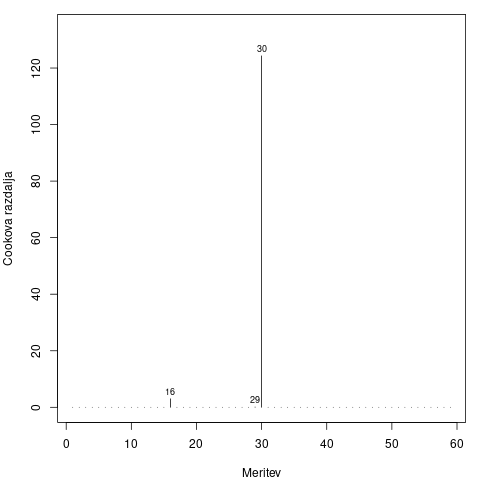
\includegraphics[width=1\textwidth]{res/netrans-vpliv-tock-na-model.png}
        \captionof{figure}{Vpliv točk na model\\(netransformiran)}
        \label{img:netrans-vpliv-tock-na-model}
    \end{subfigure}
    \caption{Netransformirani diagnostični grafi}
    \label{img:netrans-diagnosticni-grafi}
\end{figure}

Koda za generiranje diagnostičnih grafov je bolj podrobno predstavljena v poglavjih \ref{sec3} in \ref{sec5}.